\section{גישת הפתרון}

כדי להתמודד עם האתגר של חיזוי משתנים ביו-כימיים מורכבים בבית השורשים, פותחה גישה מערכתית המבוססת על שרשרת חיזוי דו-שלבית. גישה זו מפרקת את הבעיה לשני שלבים מרכזיים: תחילה חיזוי ותיאור תנאי המיקרו-אקלים בתוך החממה, ולאחר מכן חיזוי תגובת בית השורשים על בסיס תנאים אלו, פעולות ההשקיה והדישון, מצב הצמח ומדידות עבר.

מבנה זה מאפשר להשתמש בנתונים זמינים יחסית, כגון אקלים חיצוני, השקיה, דישון ומדידות ידניות קודמות, כדי להעריך את ערכי ה-pH וה-EC גם בפרקי הזמן שבהם לא קיימת מדידה ישירה של בית השורשים.

\subsection{מסד הנתונים}
המחקר מתבסס על נתונים אגרו-מטאורולוגיים ותפעוליים שנאספו במהלך עונת הגידול 2025, בין החודשים מאי לספטמבר. לצורך אימון ובדיקת המודלים נבנה מסד נתונים מאוחד (Master) המשלב מקורות מידע הטרוגניים לאחר תהליכי ניקוי, סנכרון ואיחוד לזמן אחיד.

מסד הנתונים הסופי נבנה ברזולוציה של 10 דקות וכלל 16{,}682 רשומות, בטווח התאריכים 29.05.2025 עד 21.09.2025. הנתונים נחלקים לשתי קבוצות עיקריות:

\begin{itemize}
    \item \textbf{נתונים רציפים:} נתונים שנמדדו בתדירות גבוהה ממקורות כגון תחנה מטאורולוגית חיצונית ולוגר נתונים פנימי בחממה. נתונים אלו כוללים משתנים כגון קרינה, טמפרטורה, לחות יחסית, מהירות רוח, טמפרטורת קרקע והתאדות פוטנציאלית.
    \item \textbf{נתונים בדידים ודלילים:} מדידות ידניות של ערכי pH ו-EC בבית השורשים. מדידות אלו משמשות כערכי היעד של המודל, אך הן דלילות ביחס לנתוני האקלים והתפעול. בסך הכול היו 109 נקודות מדידה מתויגות של pH ו-EC.
\end{itemize}

פער זה בין נתונים רציפים וצפופים לבין מדידות יעד דלילות היווה את אחד האתגרים המרכזיים בפרויקט. לכן, המודל לא נבנה כחיזוי פשוט של כל נקודת זמן, אלא כחיזוי שינוי בין נקודת בסיס ידועה $t_0$ שבה קיימת מדידת pH ו-EC לבין נקודת יעד עתידית $t_1$.

\subsection{השלמת נתונים היסטוריים \LR{(Data Imputation using LightGBM)}}
אחד האתגרים בפרויקט היה חוסר רציפות בחלק מנתוני המיקרו-אקלים בתוך החממה. כדי להימנע מאובדן תקופות שבהן קיימות מדידות בית שורשים אך חסרים נתוני אקלים פנימי, פותחו מודלים לחיזוי משתני מיקרו-אקלים על בסיס נתוני אקלים חיצוניים.

מודלים אלו למדו את הקשר בין תנאי האקלים מחוץ לחממה לבין התנאים בתוך החממה, כגון טמפרטורה, לחות, קרינה פנימית והתאדות. בדרך זו ניתן היה להשלים או לחזות משתנים פנימיים הדרושים למודל בית השורשים, ולהגדיל את כמות המידע הזמין עבור שלב החיזוי המרכזי.

\begin{figure}[H]
    \centering
    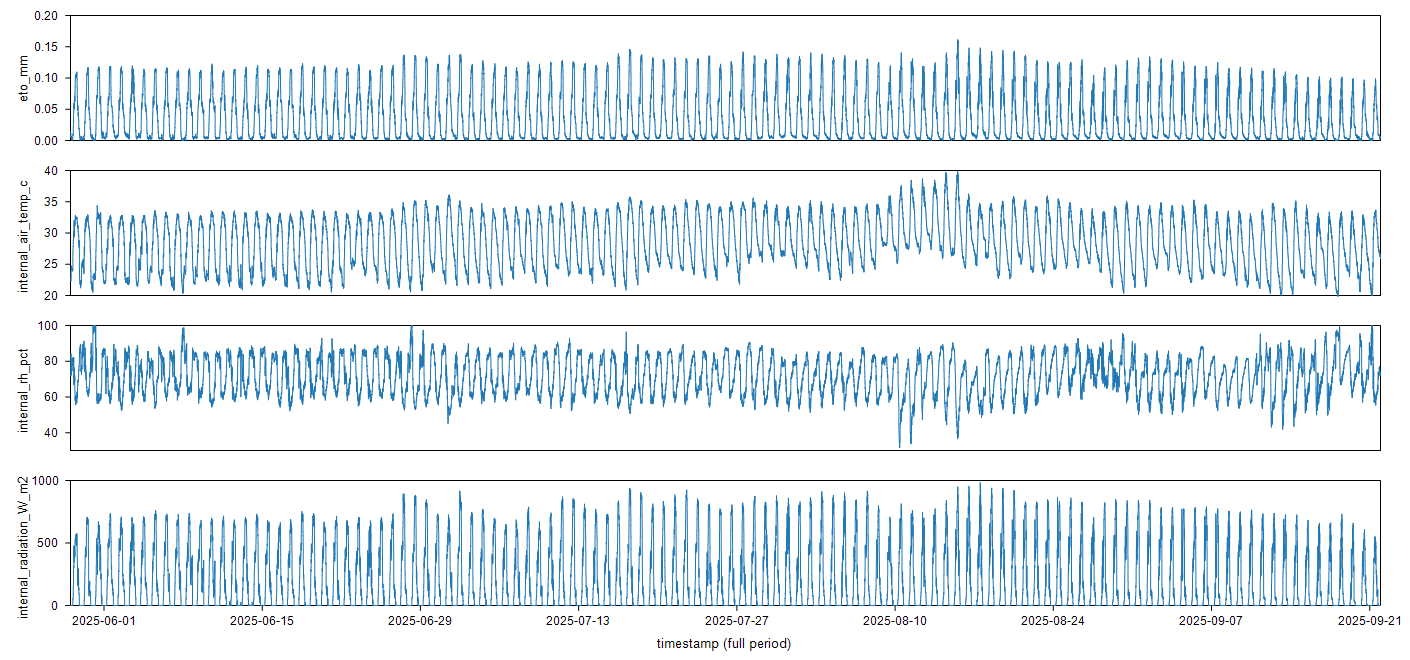
\includegraphics[width=\textwidth]{figures/fig04.png}
    \caption{\LR{Historical Microclimate Data Imputation Results}}
    \label{fig:imputation}
\end{figure}

איור \ref{fig:imputation} מציג את סדרות הזמן של משתני המיקרו-אקלים (ET0, טמפרטורה פנימית, לחות יחסית וקרינה פנימית) לאורך כל תקופת הניסוי, לאחר תהליך ההשלמה.

\subsection{עיבוד מקדים}
לפני שלב האימון בוצע עיבוד מקדים לנתונים, שכלל ניקוי ערכים חריגים או לא פיזיקליים, טיפול בחוסרים, וסנכרון זמני המדידה בין מקורות המידע השונים.

בנוסף, לכל מרווח חיזוי בין $t_0$ ל-$t_1$ הוצמדה היסטוריית התנאים שהתרחשה בין שתי הנקודות. כלומר, עבור כל דגימת יעד של pH ו-EC חושבו משתני אקלים, השקיה, דישון ומצב צמח המתארים את התהליך שהוביל מהמצב ההתחלתי למצב העתידי.

\subsection{ארכיטקטורת המערכת}
המערכת בנויה כשני שלבים עיקריים:

\textbf{שלב 1: מודל מיקרו-אקלים.} שלב זה נועד לתרגם את תנאי האקלים החיצוניים לתנאים הצפויים בתוך החממה. המודל מקבל כקלט משתנים כגון קרינה, טמפרטורה, לחות ומהירות רוח, ומפיק הערכה של משתני מיקרו-אקלים פנימיים, כגון טמפרטורה, לחות, קרינה פנימית והתאדות. הרציונל הוא שבית השורשים מושפע מהתנאים בתוך החממה ולא רק מתנאי הסביבה החיצונית. לכן, שלב זה מאפשר להשתמש במידע מטאורולוגי זמין כבסיס לחיזוי מדויק יותר של סביבת הגידול בפועל.

\textbf{שלב 2: מודל בית השורשים.} זהו מודל הליבה של הפרויקט. המודל מקבל כקלט את ערכי ה-pH וה-EC בנקודת הבסיס, את תנאי המיקרו-אקלים, את נתוני ההשקיה והדישון, את מצב הצמח ואת משך הזמן בין $t_0$ ל-$t_1$. על בסיס מידע זה הוא חוזה את ערכי ה-pH וה-EC בנקודת הזמן העתידית.

בשלב הסופי פותח מודל היברידי, המשלב בין רכיב \GB{} לבין רכיב ליניארי חסין. רכיב ה־\GB{} נועד ללמוד דפוסים מורכבים ולא ליניאריים מתוך נתוני העבר, בעוד שהרכיב הליניארי מסייע בהתמודדות עם מגמות ואירועים תפעוליים בעלי השפעה גבוהה. שילוב זה מאפשר למודל לבצע גם אינטרפולציה בתוך דפוסים מוכרים וגם אקסטרפולציה זהירה במצבים חריגים יותר.

\begin{figure}[H]
    \centering
    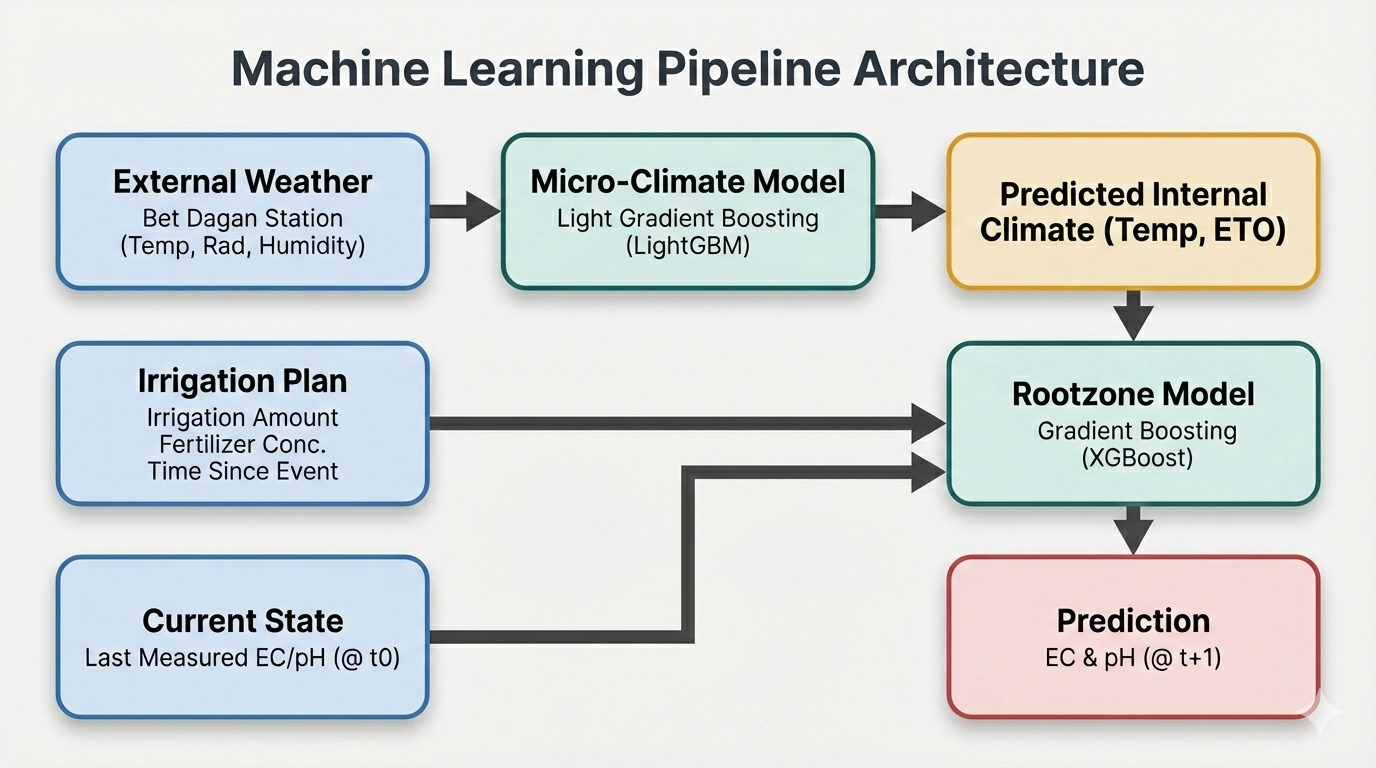
\includegraphics[width=0.8\textwidth]{figures/fig06.png}
    \caption{\LR{System Architecture -- Two-Stage Prediction Architecture}}
    \label{fig:architecture}
\end{figure}

איור \ref{fig:architecture} ממחיש את זרימת המידע בין שני השלבים: נתוני מזג האוויר החיצוני עוברים דרך מודל המיקרו-אקלים (LightGBM), ותוצאתו, יחד עם תוכנית ההשקיה והמצב ההתחלתי, מוזנת למודל בית השורשים (XGBoost) המפיק את התחזית הסופית.

\subsection{אסטרטגיית איחוד הנתונים}
אחד האתגרים המרכזיים בפרויקט היה השוני ברזולוציית הזמן בין מקורות הנתונים. נתוני האקלים והלוגר נאספו בתדירות גבוהה של 10 דקות, בעוד שמדידות pH ו-EC בוצעו באופן ידני ובתדירות נמוכה בהרבה.

כדי להתמודד עם פער זה, נבנה \LR{Master Dataset} בציר זמן אחיד של 10 דקות. הנתונים הרציפים נשמרו ברזולוציה המקורית, ואילו מדידות ה-pH וה-EC שימשו כנקודות יעד בלבד. מודל בית השורשים אומן על מרווחים שבהם קיימת מדידת בסיס ומדידת יעד, ולא על כל נקודת זמן בנפרד.

\begin{figure}[H]
    \centering
    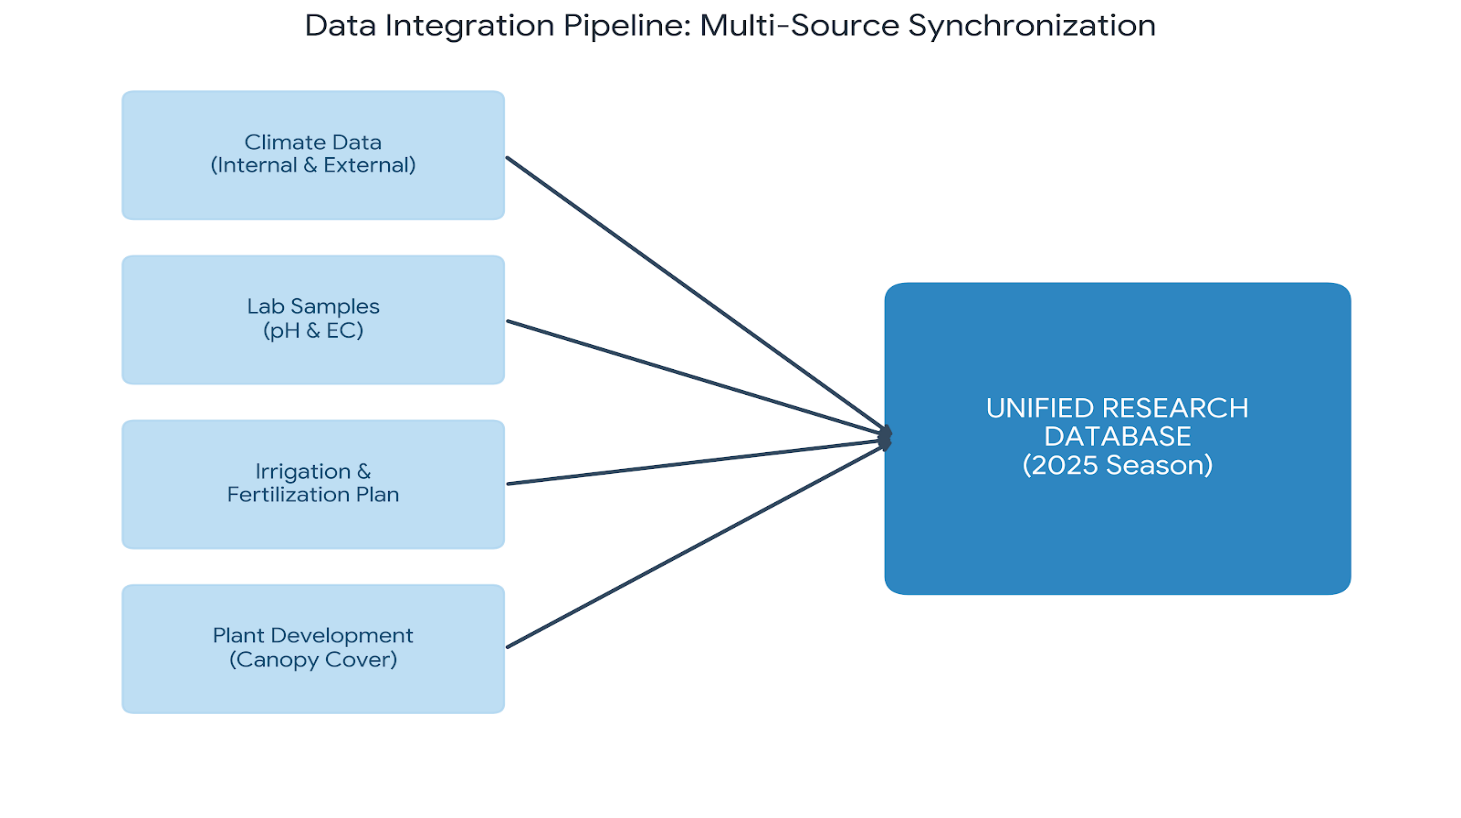
\includegraphics[width=0.8\textwidth]{figures/fig05.png}
    \caption{\LR{Data Integration Pipeline -- Unified Master Dataset Construction}}
    \label{fig:pipeline}
\end{figure}

גישה זו, המתוארת באיור \ref{fig:pipeline}, מאפשרת למודל ללמוד את השינוי שהתרחש בבית השורשים לאורך מרווח זמן נתון, במקום לנסות לחזות ערך רגעי ללא מדידת אמת תואמת.

\subsection{הנדסת פיצ'רים \LR{(Feature Engineering)}}
כדי לאפשר למודל ללמוד את התהליכים האגרונומיים והפיזיקליים המשפיעים על בית השורשים, נבנו משתנים חדשים מתוך הנתונים הגולמיים.

\begin{itemize}
    \item \textbf{משתני מצב התחלתי:} ערכי pH ו-EC בנקודת הבסיס $t_0$ המשמשים כעוגן לחיזוי.
    \item \textbf{משתני אופק חיזוי:} משך הזמן בין נקודת הבסיס לנקודת היעד, המבטא את פרק הזמן שבו הצטברו השפעות האקלים, ההשקיה והדישון.
    \item \textbf{משתני צבירה:} סכומי קרינה, התאדות, השקיה ודישון בפרקי זמן שונים. משתנים אלו מייצגים את "הזיכרון" המצטבר של המערכת.
    \item \textbf{משתני אירועים:} זמן מאז השקיה, דישון או אירוע תפעולי אחר. משתנים אלו חשובים לזיהוי תגובות מושהות של בית השורשים.
    \item \textbf{משתני מצב הצמח:} כיסוי נוף וגיל הצמח, המשמשים כאינדיקציה לגודל הצמח, קצב הדיות וצריכת המים והדשן.
\end{itemize}

\subsection{אסטרטגיית אימון ובדיקה \LR{(Walk-Forward Validation)}}
מאחר שהנתונים הם סדרה עיתית, לא נעשה שימוש בחלוקה אקראית רגילה לסט אימון וסט בדיקה, כדי למנוע זליגת מידע מהעתיד לעבר. במקום זאת יושמה שיטת \WFV{}.

בשיטה זו, המודל מאומן בכל שלב על נתוני העבר בלבד ונבחן על נקודות עתידיות. לאחר מכן חלון האימון מתקדם בזמן, והמודל נבחן שוב. תהליך זה מדמה תרחיש תפעולי שבו בכל נקודת זמן זמינים למודל רק הנתונים שנאספו עד אותה נקודה.

\begin{figure}[H]
    \centering
    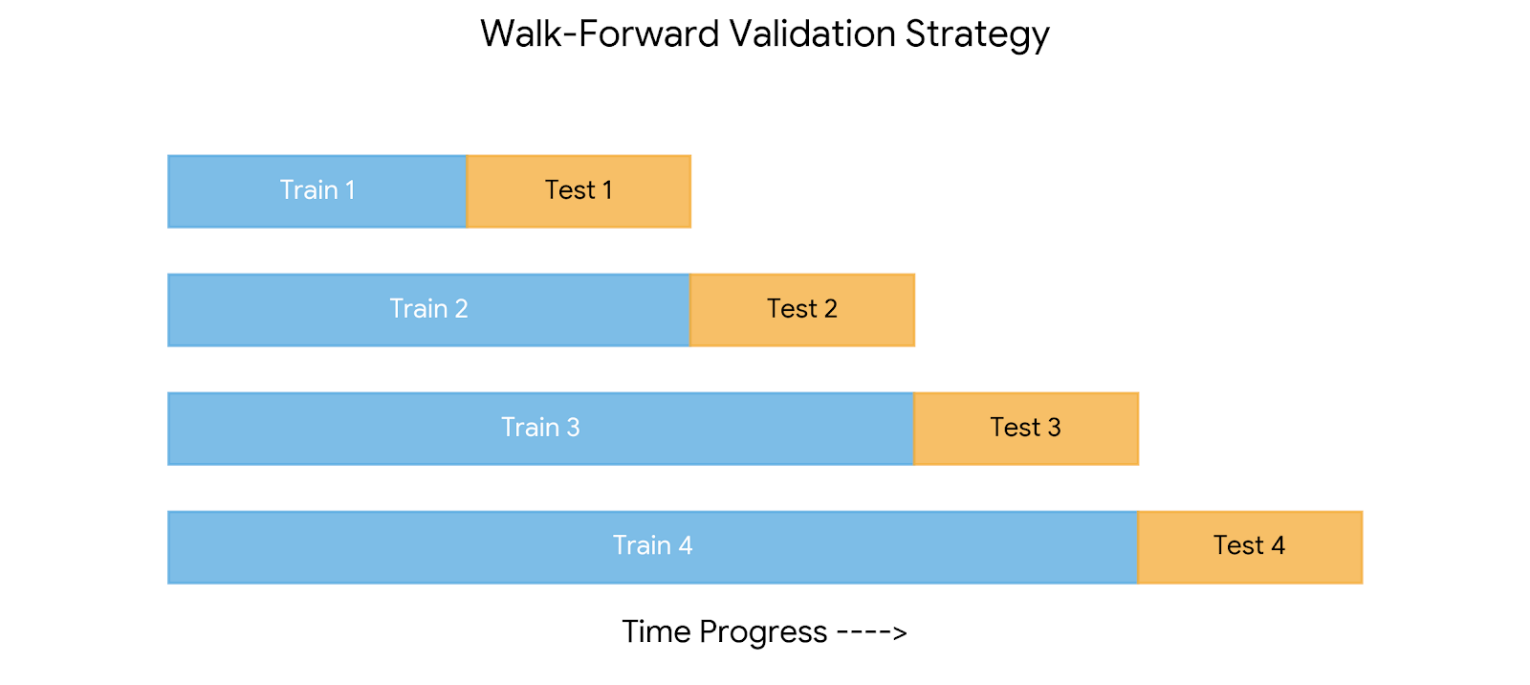
\includegraphics[width=0.8\textwidth]{figures/fig07.png}
    \caption{\LR{Walk-Forward Validation Strategy}}
    \label{fig:walkforward}
\end{figure}

כפי שמתואר באיור \ref{fig:walkforward}, בכל איטרציה מתרחב חלון האימון, ואילו חלון הבדיקה מתקדם בזמן -- כך שהמודל תמיד נבחן על נתונים עתידיים ביחס לחלון האימון שלו.

בנוסף, בוצעה בדיקת Holdout על מרווחים מדולגים, שבה חלק מהמרווחים הוצאו מתהליך האימון ושימשו לבדיקת יכולת ההכללה של המודל. בדיקה זו נועדה לבחון האם המודל מסוגל לחזות נקודות שלא שימשו ללמידה, ולא רק לשחזר דפוסים מתוך נתוני האימון.

בפרויקט נבחנו גרסאות חיזוי שונות, ובהן גרסת 24 שעות וגרסת 48 שעות. הגרסה הסופית מדגישה את יכולת המודל לחזות את תגובת בית השורשים בטווח של עד 48 שעות, תוך שמירה על מבנה בדיקה המדמה שימוש עתידי במערכת תומכת החלטה.
